% !TeX spellcheck = pt_PT
%

\chapter{Aplicação Cliente} \label{cliente}

Este capítulo vai apresentar a nossa solução para o lado da aplicação cliente.

\section{Introdução e Estrutura da Aplicação Cliente} \label{sec41}
A aplicação cliente é a segunda partição do nosso projeto. É a partição onde se encontra a interface de utilizador, painéis de controlo e alguma lógica de negócio adicional.

Foram geradas na aplicação cliente as classes correspondentes às Entidades da aplicação servidora em \emph{TypeScript}. Podemos observar no troço de código seguinte, como exemplo, a classe \emph{Event.ts} inserida no \emph{package} de classes da nossa Aplicação Cliente.

\begin{lstlisting}
 import {Profile} from './profile';

 export class Event {
 	constructor(
		private id?: number,
		private name?: string,
		private description?: string,
		private date?: Date,
		private local?: string,
		private profiles?: Profile[]
 	) {
		this.id = id ? id : 0;
		this.description = description ? description : '';
		this.date = date ? date : new Date(0);
		this.local = local ? local : '';
		this.name = name ? name : '';
		this.profiles = profiles ? profiles : [];
	  }
 }
\end{lstlisting}

Um dos aspetos principais a salientar na implementação dos construtores das Entidades na aplicação cliente é a questão das propriedades poderem ser \emph{nullable}. Organizando os construtores para que todas as propriedades sejam \emph{nullable} enquanto se faz a verificação no corpo do construtor para a ausência destas propriedades, permite-se construir objetos atribuindo valores padrão a todas as propriedades que não existem na altura da criação. Este detalhe de implementação ajuda a gerar objetos vazios sem os problemas que ocorrem frequentemente na manipulação de valores \emph{null}.


O tipo de organização e estrutura de uma aplicação cliente que o \emph{Angular} incentiva a aplicar é a estrutura \emph{Component} - \emph{Service}, e é esta estrutura que é seguida no nosso projeto.\\

\subsection{\textit{Angular Component}}\label{sub411}

Um \emph{Component} em \emph{Angular} é uma peça visual de uma aplicação, que pode estender deste uma página a uma tabela ou a um \textit{menu}. Não existe qualquer requisito sobre que tipo de objeto o componente representa, e esse tipo é meramente para fins de organização da aplicação. 

No caso da nossa aplicação cliente, cada especificação principal tem o seu \emph{endpoint} e consequentemente o seu \emph{Component}. Dado que algumas regras de negócio implicam que certos \emph{endpoints} necessitem de componentes adicionais, como as estruturas \emph{Modal} ou \emph{Pop-over} que existem na \emph{Ionic Framework} (explicadas em detalhe na sub-secção 4.1.4), foi tomada como regra de decisão gerar estas estruturas num \emph{Component} separado do \emph{Component} das páginas dos \emph{endpoints}, que são invocados nas circunstâncias apropriadas.\\
Cada \textit{Component} tem associado um \textit{template}, que representa o ficheiro \textit{HTML} com a vista do componente, e um ficheiro \textit{TypeScript} que representa a instância da classe do próprio \textit{Component}, onde se encontram as definições das estruturas de dados internas do \textit{Component}, os \textit{imports} necessários ao \textit{Component}, assim como métodos chamados pelo \textit{template} com alguns comportamentos visuais, como os métodos invocados pelos eventos de \textit{click} de um botão ou \textit{check}/\textit{uncheck} de uma \textit{checkbox}, métodos que chamam os serviços que fazem o \textit{data-fetching}, métodos de \textit{redirect} da página, ou métodos que invocam os \textit{Controllers} dos componentes adicionais mencionados anteriormente.
Cada Component tem também o seu \textit{NgModule}. \textit{NgModules} são um tipo de estrutura disposta no \textit{Angular}, que ajuda a organizar a aplicação em módulos que podem ser importados ou importar outros módulos. A nossa aplicação cliente está assim estruturada para cada \textit{Component} ter o seu próprio módulo (os componentes adicionais são inseridos no mesmo módulo que o componente a que estão contextualmente associados), assim como o seu próprio \textit{routing module}, inserido dentro do módulo do componente, que trata do \textit{routing} dentro do módulo. Esta abordagem permite-nos ter o \textit{routing} todo da aplicação re-partido pelos módulos, em vez de estar todo centralizado num único componente.

\newpage

\subsection{\textit{Angular Service}}\label{sub412}

Típicamente em arquitetura de \emph{software}, o termo \emph{Service} (ou serviço) é um termo utilizado para denominar uma peça de \emph{software} que tem um conjunto de funcionalidades expecíficas e limitadas, que estão por norma ligadas e contextualizadas, e que podem ser utilizadas e re-utilizadas por diferentes partes de uma aplicação. 

No caso do \emph{Angular}, um \textit{Service} não é mais que uma classe onde são escritas funcionalidades, e que pode ser anotada como \emph{@Injectable} para que o \textit{Angular} consiga injectar essas funcionalidades num \textit{Component} através de um \textit{injector}. 

No caso da nossa aplicação cliente, cada entidade dispõe de um serviço \textit{HttpService} (agrupados no \textit{package} \textit{app/httpservices}) que contem todos os métodos que fazem as chamadas feitas à \textit{web API} exposta pela aplicação servidora. 

Podemos observar no troço de código seguinte, como exemplo, o serviço \textit{HttpEventService}.

\begin{lstlisting}
	import { Injectable } from '@angular/core';
	import { HttpClient, HttpHeaders } from '@angular/common/http';
	import { Event } from '../../classes/event';
	import { Observable, throwError } from 'rxjs';
	
	@Injectable ({
		providedIn: 'root'
	})
	
	export class EventService {
		private BASE_URL = 'http://localhost:8080/event';
		private httpOptions = {
			headers: new HttpHeaders({
			'Content-Type':  'application/json',
			Authorization: 'my-auth-token',
			'Access-Control-Allow-Origin': '*'
			})
		};
	
		constructor(private http: HttpClient) { }
		
		getEvents(): Observable<Event[]> {
			const url = `${this.BASE_URL}/all`;
			return this.http.get<Event[]>(url, this.httpOptions);
		}
		
		getEventsById(id: any) {
			const url = `${this.BASE_URL}/findById/${id}`;
			return this.http.get(url, this.httpOptions);
		}
		
		postEvent(event: Event): Observable<Event> {
			const url = `${this.BASE_URL}/post`;
			return this.http.post(url, event, this.httpOptions);
		}
		
		updateEvent(event: Event): Observable<any> {
			const url = `${this.BASE_URL}/update`;
			return this.http.put(url, event, this.httpOptions);
		}
		
		deleteEvent(id: number): Observable<any> {
			const url = `${this.BASE_URL}/delete/${id}`;
			return this.http.delete(url, this.httpOptions);
		}
}
\end{lstlisting}

Certas entidades dispõe tambem de um serviço próprio(agrupados no \textit{package} \textit{app/componentservices}) que contem todos os métodos que envolvem a algoritmia de regras de negócio adicionais dessas entidades. 
Podemos observar no troço de código seguinte, como exemplo, o serviço \textit{AthleteGameStatsService}, que contem um método \textit{getTotal()}, que retorna um objeto \textit{Stats} com o somatório de todos os \textit{Stats} dentro do array de \textit{AthleteGameStats}, utilizado na geração da tabela de estatísticas de um atleta. 

\begin{lstlisting}

	import { Injectable } from '@angular/core';
	import { AthleteGameStats } from "../../classes/associations/AthleteGameStats";
	import { Stats } from "../../classes/stats";
	
	@Injectable ({
		providedIn: 'root'
	})
	
	export class AthleteGameStatsService {
	
		constructor() { }
	
		getTotal(stats: AthleteGameStats[]) {
			let acc: Stats = new Stats();
			Object.keys(acc).forEach( key => {
				stats.forEach( stat => {
					acc[key] += stat.stats[key];
				});
			});
			return acc;
		}
	}
}
\end{lstlisting}

\newpage

\subsection{\textit{Angular Data Binding}}\label{subsec413}

O \textit{Angular} também dispõe de um sistema de sintaxe de \textit{templates} que é utilizado com regularidade ao longo da aplicação. Dado que cada \textit{Component} tem a sua instância de classe e \textit{template} com a sua vista, o \textit{Angular} permite que estas vertentes comuniquem uma com a outra programáticamente através do chamado \textit{Data Binding}. 
Os principais tipos de \textit{Data Binding} que existem no \textit{Angular} são \\

\begin{tabular}{ll}
	\emph{Interpolation} & Corresponde a ligar uma expressão que é calculada quando o \textit{template} é \\
	& gerado a um elemento \textit{HTML} dentro desse \textit{template}. \\
	& A sintaxe deste \textit{binding} é {\{\{\textit{expression}\}\}}. \\
	\\
	\emph{Property} & Corresponde a ligar uma propriedade do \textit{Component} a um elemento \textit{HTML} do \\
	& \textit{template}. É uma ligação denominada \textit{Source-to-View}, que altera dinâmicamente \\
	& o valor do elemento para o valor da propriedade, mesmo quando o valor da \\
	&propriedade é alterado em \textit{run-time}. \\
	& A sintaxe deste \textit{binding} é [\textit{target}]="\textit{expression}".\\
	\\
	\emph{Event} & Corresponde a ligar um evento de um elemento \textit{HTML} a uma declaração do \\
	& \textit{Component}. É uma ligação denominada \textit{View-to-Source}, que conecta um evento \\
	&na vista (\textit{click} de um botão, \textit{check}/\textit{uncheck} de uma \textit{checkbox}) a uma declaração \\
	&(podendo ser um método do \textit{Component}). \\
	& A sintaxe deste \textit{binding} é (\textit{target})="\textit{statement}".\\
	\\
	\emph{Two-Way} & Corresponde a uma ligação dupla entre uma propriedade e um elemento. \\
	& O valor da propriedade transita até ao elemento, onde este pode ser alterado \\
	&através da interação do utilizador, e o novo valor transita de volta até à \\
	&propriedade. Esta ligação é normalmente usada em Formulários. \\
	&A sintaxe deste binding é [(\textit{target})]="\textit{expression}".\\
	\\
\end{tabular}

\newpage

O \textit{Angular} também contem alguns tipos de \textit{binding} especializados para estilos. Estes tipos de \textit{binding} são utilizados quando se quer alterar programaticamente alguns aspetos visuais do \textit{template} sem querer fazer essa ligação a propriedades no \textit{Component}. Estes tipos especializados são\\

\begin{tabular}{ll}
	\textit{Attribute} & Corresponde a ligar um atributo a um elemento \textit{HTML} do \textit{template}. \\
	&Este tipo de ligação é pouco usual, porque é normalmente preferível fazer uma ligação\\
	& de uma propriedade ao elemento. Mas em certos casos (por exemplo, quando se utiliza \\
	&ARIA - Accessible Rich Internet Applications , ou SVG - Scalable Vector Graphics),\\
	& o objetivo da ligação não é ligar uma propriedade ao elemento, visto que não existe \\
	&uma propriedade neste contexto onde fazer a ligação, mas sim alterar atributos do \\
	&elemento. Neste caso, utiliza-se o \textit{Attribute Binding}. \\
	&A sintaxe deste \textit{binding} é igual ao \textit{Property Binding},\\ &substituindo o nome da propriedade pelo nome do atributo \\
	&[\textit{attr.atribute-name}]="\textit{expression}".\\
	\\
	\textit{Class} & Corresponde a ligar uma classe \textit{CSS} a um elemento \textit{HTML} do \textit{template}. \\
	&Esta ligação é usada quando se quer que um elemento do template possa ter dois tipos \\
	&de classes \textit{CSS}, alternaveis em \textit{run-time} pelo valor de uma expressão. \\
	& A sintaxe deste \textit{binding} é igual ao \textit{Property Binding},\\
	& substituindo o nome da propriedade pelo nome da classe\\
	& \textit{CSS} [\textit{class.name}]="\textit{expression}".\\
	\\
	\textit{Style} & Corresponde a ligar um estilo expecífico a um elemento \textit{HTML} do \textit{template}. \\
	& No contexto do nosso projeto, este \textit{binding} é utilizado no formulário de adição de \\
	&estatísticas de um atleta, onde o valor de uma estatística demonstra gradualmente 
	\\
	&através de cores diferentes o carácter do valor (cores na gama do azul e verde são\\
	& consideradas cores positivas, apresentadas em estatísticas com valores com percentagem \\
	&de sucesso acima dos 50\%, enquanto que cores na gama do laranja e vermelho são\\
	& consideradas cores negativas, apresentadas em estatísticas com valores com percentagem \\
	&de sucesso abaixo dos 50\%). \\
	& A sintaxe deste binding é igual ao Property Binding,\\
	& substitundo o nome da propriedade pelo nome do estilo [\textit{style.name}]="\textit{expression}";\\
\end{tabular}
\\

\subsection{\textit{IONIC API}}\label{subsec414}

A \textit{API} do \textit{Ionic} dispõe de uma lista de vários componentes visuais que podem ser intercalados com os do \textit{Angular} para criar uma aplicação responsiva e adaptável ao dispositivo em que é executada. Em [1] podemos encontrar a lista completa de todos os componentes disponíveis na \textit{API} do \textit{Ionic}. Ao longo deste projeto foram usados diversos componentes, nos casos que foram considerados apropridados, para garantir que eram cumpridas todas as regras de negócio aplicáveis, assim como garantir que a interface do utilizador seja clara e explícita na sua utilização.
Ao longo do desenvolvimento da aplicação cliente, foram utilizados diversos componentes em diversos contextos. No que toca a menus, foram utilizados\\

\begin{tabular}{ll}
	\textit{ion-split-pane} & Menu lateral que aparece constantemente em toda a aplicação, onde se \\
	& encontram ligações para as diversas páginas, e se esconde automáticamente \\
	& quando o tamanho do écran é menor que um determinado \textit{threshold}, ou se \\
	& esconde manualmente em algumas páginas que apresentam elementos de \\
	&grande dimensão (ex.: a tabela de \textit{AthleteGameStats}).\\
	\\
	\textit{ion-tabs} & Barra de navegação, que aparece no \textit{footer} da página, com \textit{icons} com \textit{routing} \\
	&para todas as páginas da aplicação. Apesar de indicar alguma redundância \\
	& quando utilizado em conjunto com o \textit{ion-split-pane}, em contextos onde este \\
	&colapsa, como referido anteriormente, o \textit{ion-tabs} torna-se o menu que melhor \\
	&facilita a navegação pela aplicação. Este menu é lateralmente \textit{scrollable}, \\
	&tornando-o extremamente responsivo em qualquer tipo de dispositivo.\\
	\\
	\textit{ion-header} & Barra de navegação, que aparece no \textit{header} da página, com uma \textit{ion-toolbar} \\
	&onde podem ser inseridos botões ou segmentos. No contexto da nossa aplicação \\
	&cliente, dependendo da página, este componente tem por norma um \textit{back button}, \\
	&botão de adicionar um elemento, botão de informação sobre a página e título \\
	&da página. No caso do calendário, tem botões para o filtro e para a barra \\
	&de procura, e em outros casos, segmentos com abas para os diversos tipos de \\
	&informação a mostrar (calendário com \textit{Upcomming}, \textit{All} e \textit{Past}, \\
	&estatísticas com \textit{Stats} ou \textit{Graph}).\\
\end{tabular}

\begin{figure}[h]
	\begin{center}
		\resizebox{150mm}{!}{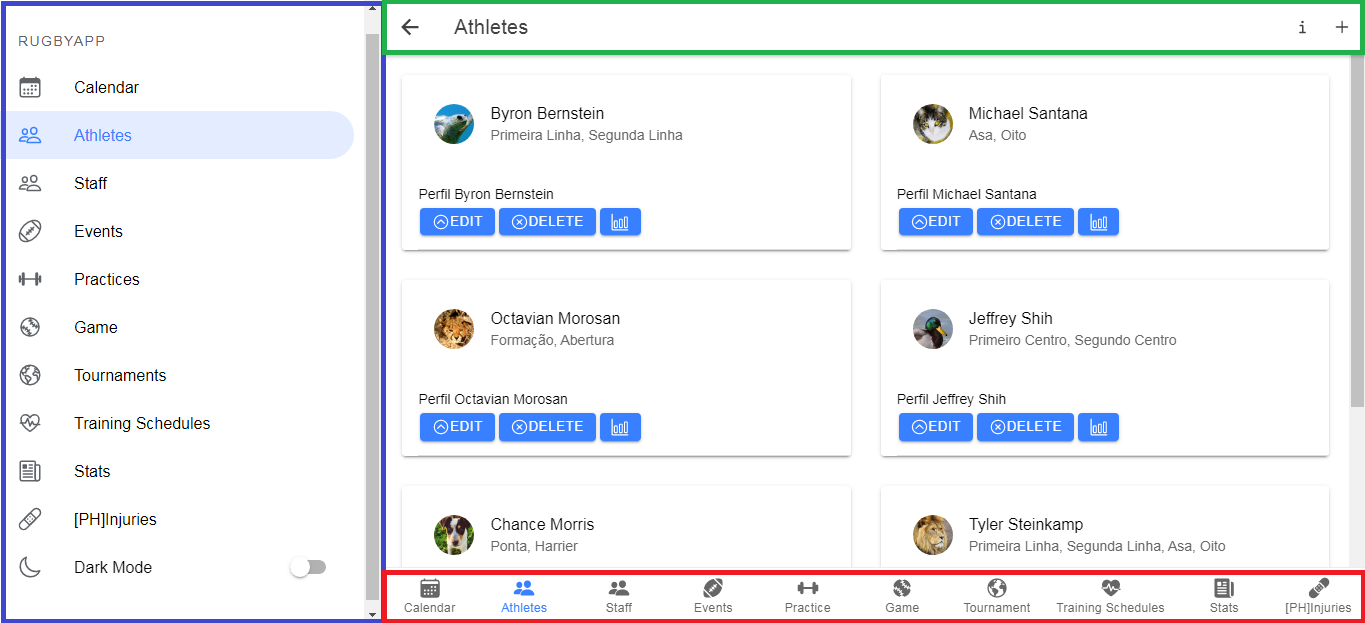
\includegraphics{./figures/frontend/MainComponent.png}}
	\end{center}
	\caption{Figura da vista inicial da aplicação. Observa-se o \textit{ion-split-pane} a azul, o \textit{ion-tabs} a vermelho e o \textit{ion-heasder} a verde.}\label{fig:maincomponent}
\end{figure}
\pagebreak

Como mencionado na secção 4.1.1, existem \textit{endpoints} na nossa aplicação cliente que requerem mais do que um \textit{Component} para garantir certas regras de negócios sem que a informação nas páginas fique sobrelotada e proporcionando a melhor experiência de utilização. Existem componentes na \textit{API} do \textit{Ionic} (alguns também mencionados na secção 4.1.1) que foram utilizados para este mesmo propósito\\

\begin{tabular}{ll}
	\textit{ion-modal} & \textit{Dialog} (componente visual que se sobrepõe ao contexto atual da página e \\
	&requer interação do utilizador para desaparecer), normalmente utilizado \\
	&para apresentar uma página onde o utilizador tem diversas opções de interação.\\
	& É utilizado no formulário de \textit{Practices} para o utilizador escolher na folha de \\
	&presenças os diversos tipos de treino suportados pelo nosso modelo que o \\
	&atleta realizou.\\
	\\
	\textit{ion-popover} & \textit{Dialog} (assim como o \textit{ion-modal}) que é geralmente usado para conter acções \\
	&ou informação que não pode ser mostrada na totalidade sem comprometer\\
	& visualmente os elementos da página. É utilizado nas diversas tabelas com \\
	&a lista de \textit{Events}, \textit{Games}, \textit{Tournaments}, \textit{Practices}, etc, para "esconder" a lista \\
	&de presenças atrás de um botão, para que as listas fiquem mais organizadas \\
	&e visualmente "limpas".\\
	\\
	\textit{ion-select} & Apesar de não requirir um \textit{controller} ou um \textit{component} próprio para ser \\
	&programado, o \textit{ion-select} é um \textit{ion-modal} pré-definido na \textit{API} exclusivamente \\
	&para \textit{input}/\textit{output} (ou seja, não é possível atribuir-lhe diretamente outro \\
	&comportamento que não o de dar ao utilizador diversas opções, das quais este \\
	&escolhe uma ou várias, dependendo do contexto, e o \textit{ion-select} junta-as e \\
	&guarda-as numa \textit{string}). É utilizado nos nossos formulários para dar ao \\
	&utilizador uma lista de escolhas possíveis, com que ele possa interagir para \\
	&fazer as suas escolhas.
\end{tabular}

\begin{figure}[h]
	\begin{center}
		\resizebox{150mm}{!}{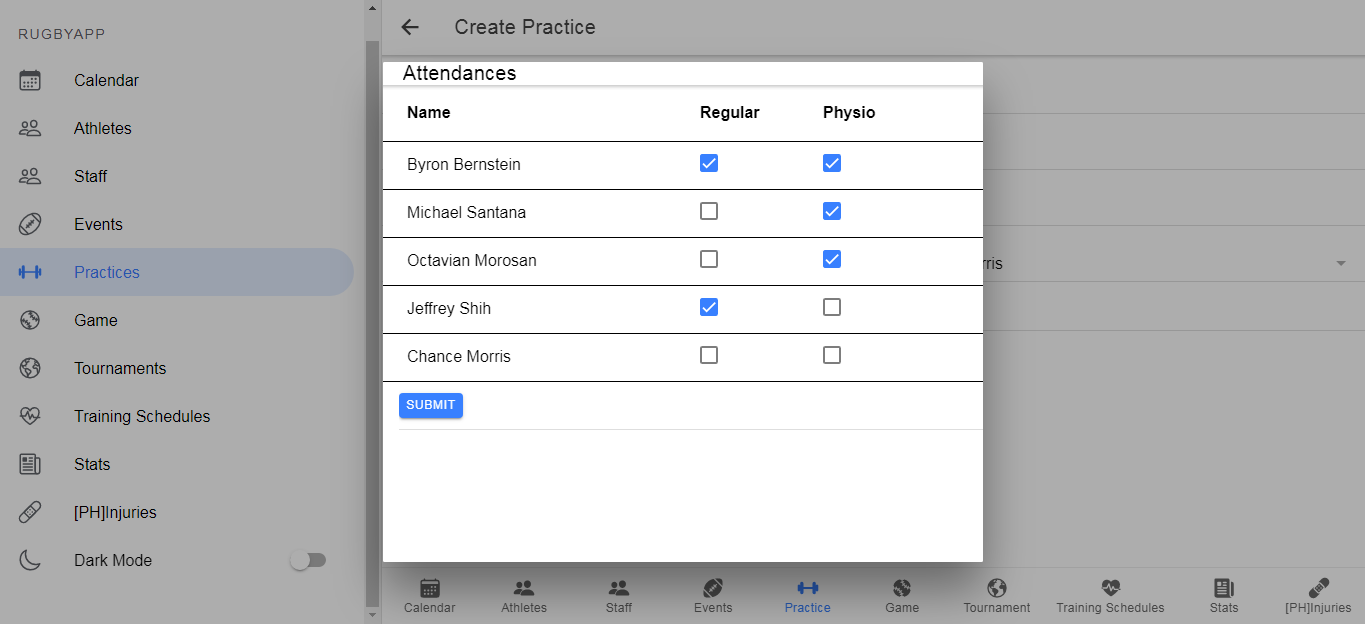
\includegraphics{./figures/frontend/PracticeFormPopover.png}}
	\end{center}
	\caption{Figura do \textit{Modal} do \textit{endpoint} do formulário de \textit{Practice}.}\label{fig:practiceformmodal}
\end{figure}
\newpage

\begin{figure}[h]
	\begin{center}
		\resizebox{150mm}{!}{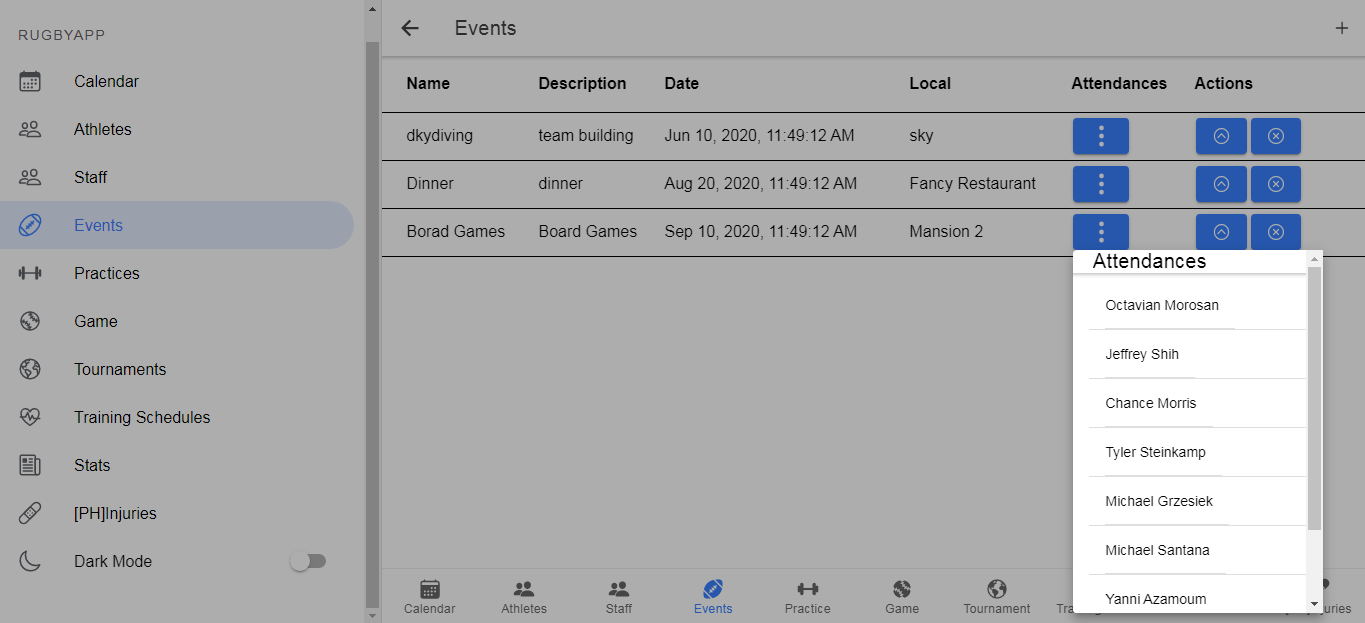
\includegraphics{./figures/frontend/EventPopover.png}}
	\end{center}
	\caption{Figura do \textit{Popover} do \textit{endpoint Event}.}\label{fig:eventpopover}
\end{figure}

\begin{figure}[h]
	\begin{center}
		\resizebox{150mm}{!}{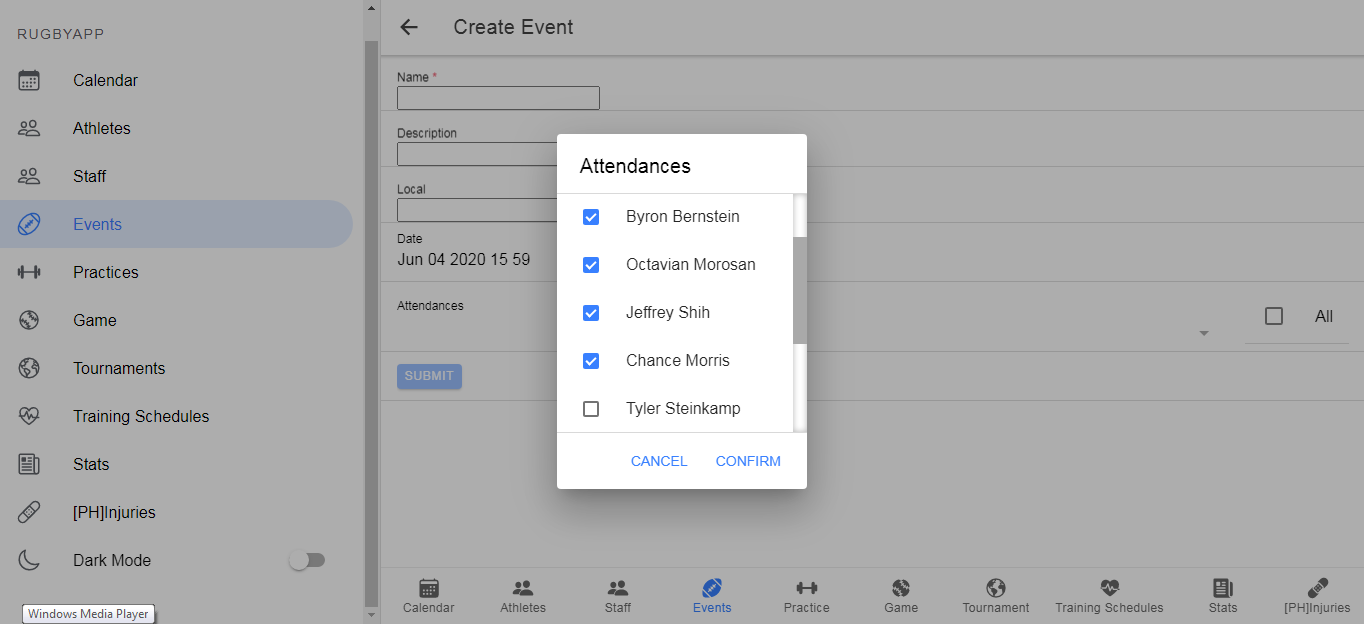
\includegraphics{./figures/frontend/EventFormSelect.png}}
	\end{center}
	\caption{Figura do \textit{Select} do \textit{endpoint} do formulário de \textit{Event}.}\label{fig:eventformselect}
\end{figure}
 \newpage
 
Como referido anteriormente, ao contrário do \textit{ion-select}, o \textit{ion-modal} e o \textit{ion-popover} são componentes próprios e requerem um \textit{controller} para serem gerados e criados por outros componentes. Podemos observar no troço de código seguinte, o método \textit{createPopover()} inserido no \textit{event.component}

\begin{lstlisting}
constructor(private eventService: EventService, private popoverController: PopoverController, private alertController: AlertController) { }

/* . . .*/

async createPopover(profiles: Profile[], ev) {
	const popover = await this.popoverController.create({
		component: EventPopoverComponent,
		componentProps: { profiles },
		event: ev
	});
	return await popover.present();
}
\end{lstlisting}



O \textit{Component event.component} importa o módulo \textit{PopoverController} do \textit{package} do \textit{Ionic}, e cria a sua instância no construtor. Atribuindo o método \textit{createPopover} a um evento, é assim invocada a criação de um \textit{Popover}. Passando esse mesmo evento ao método \textit{create} do \textit{controller}, fazemos com que o \textit{Popover} seja apresentado visualmente ligado ao botão que o criou, contrariamente a não ser passado um evento ao \textit{create}, que cria apenas um \textit{Popover} no topo da página.\\

\begin{lstlisting}
<ng-container matColumnDef="profiles">
	<th mat-header-cell *matHeaderCellDef> Attendances </th>
	<td mat-cell *matCellDef="let element">
		<ion-button (click)="createPopover(element.profiles,$event)">
			<ion-icon slot="icon-only" name="ellipsis-vertical"></ion-icon>
		</ion-button>
	</td>
</ng-container>
\end{lstlisting}



Cada elemento da coluna de \textit{Attendances} tem o seu próprio botão que vai criar o seu próprio \textit{Popover}. Passando a lista de \textit{Profiles} associadas a cada elemento, podemos criar um \textit{Popover} com cada uma das listas de \textit{Profiles} na tabela do \textit{endpoint Event}.\\

\begin{lstlisting}
<ion-header>
	<ion-title>Attendances</ion-title>
</ion-header>

<ion-content>
	<ion-list>
		<ion-item *ngFor="let profile of this.navParams.get('profiles')">
			<ng-template [ngIf]="profile.athlete" [ngIfElse]="staff">
				<ion-item detail="false" (click)="close()" routerLink="/app/athlete/athlete-profile/{{profile.id}}">
					<ion-label>
						<h3>{{profile.name}}</h3>
					</ion-label>
				</ion-item>
			</ng-template>
			<ng-template #staff>
				<ion-item detail="false" (click)="close()" routerLink="/app/staff/staff-profile/{{profile.id}}">
					<ion-label>
						<h3>{{profile.name}}</h3>
					</ion-label>
				</ion-item>
			</ng-template>
		
		</ion-item>
	</ion-list>
</ion-content>
\end{lstlisting}

Através de um módulo existente no package do \textit{Ionic}, chamado \textit{NavParams}, é possível passar informação ao \textit{Controller} do \textit{Popover}, e é possível do lado do \textit{Popover} obter essa informação para ser consumida. Neste caso, o Popover é meramente uma lista de itens com os nomes dos \textit{Profiles}, com um \textit{Link} para o \textit{endpoint} desse \textit{Profile}. É usado a terminologia \textit{ngIf} do \textit{Angular} para decidir entre gerar um \textit{Link} para o perfíl de um atleta ou de um \textit{staff}.

Do lado do \textit{ion-modal}, a ideia-chave é idêntica, exceto que o módulo que é importado pelo \textit{component} passa a ser o \textit{ModalController} em vez de \textit{PopoverController}. Continua-se a usar o \textit{NavParams} para passar informação ao \textit{Modal}, exceto que neste caso não se passa um evento para garantir que o \textit{Modal} fica visualmente ligado ao componente que o invocou, visto que o \textit{Modal} é sempre apresentado no meio da página.

\section{Descrição dos \textit{Endpoints}}\label{sec42}

Esta secção aborda os componentes dos diversos \textit{endpoints} implementados na aplicação cliente.


\subsection{\textit{Main Component}}\label{subsec421}

O Angular gera automaticamente um \textit{root Module}, chamado \textit{AppModule}, e um \textit{AppComponent}, que servem de raiz a todos os componentes e módulos da aplicação. O nosso AppComponent contem um 